\documentclass[12pt,twoside]{reedthesis}
\usepackage{graphicx,latexsym}
\usepackage[all]{xy}  
\usepackage{amssymb,amsthm,amsmath}
\usepackage{longtable,booktabs,setspace} 
\usepackage{url}
\usepackage{natbib}
\usepackage{marginnote}
\usepackage{listings}
\usepackage[margin=10pt,font=small,labelfont=bf]{caption} 



\newcommand{\I}{\;|\;}
\newcommand{\PR}{\mathbf{P}}
\newcommand{\E}{\mathbb{E}}
\newcommand{\Var}{\mbox{Var}}
\newcommand{\Ind}[1]{\mathbf{I}_{#1} }
\DeclareMathOperator*{\argmax}{arg\,max}

\title{Statistical Tests of Equivalence}
\author{Andrew S. Winterman}

\date{December 2010}
\division{Mathematics and Natural Sciences}
\advisor{Albyn Jones}
\department{Mathematics}

\setlength{\parskip}{0pt}

\begin{document}

\maketitle{}
  \frontmatter
  \pagestyle{empty} 


 \chapter*{Acknowledgements}
 I express my gratitude to my thesis adviser, Albyn Jones, for his insight and patient, relaxed attitude; to my family and friends, whose support helped make the thesis process far more enjoyable than I could have anticipated; and finally to Suzy Renn and the other members of the Summer 2010 Renn/Jones Lab.
 
\tableofcontents

\chapter*{Abstract}

	Tests of equivalence are motivated and described in detail. Use of tests of equivalence for microarray data analysis is described. A non-parametric bootstrap test and a t-test of equivalence are described and compared against one another via simulation. The bootstrap test, although more computationally expensive, is found to be superior, even in cases when data is normal.

  \mainmatter 
  \pagestyle{fancyplain}
  

\chapter{ Introduction }
\section{Test of Equivalence in Context}

 Tests of equivalence are a class of hypothesis tests designed to assess whether two data sets are drawn from populations whose probability distributions do not substantively differ. They are not a new statistical idea. Most commonly used by manufacturers of pharmaceuticals, tests of equivalence have found widespread use in the industry since the early 1980�s, following a 1979 Food and Drug Admistration decision stating that new, generic drugs would be approved if they could be shown to be ``bioequivalent" to existing, approved drugs \cite{wellek}. Once a drug has exhausted the duration of its patent, it can be reproduced by any company, often at a fraction of the price of the patented version. These reproductions are called ``generic" drugs. As a matter of course, both the generic and patented original version of the drug are nominally chemically identical, but they might differ in a number of ways, including milling procedure, the chemicals used in the delivery system, etc. Two drugs are bioequivalent if their action upon the body is sufficiently similar \cite{Birkett}, as demonstrated by clinical trials employing tests of equivalence. Because of the billions of dollars involved in the generic drug industry, there has been substantial theoretical attention, and many biopharmaceutical applications thoroughly described (for an exposition of such applications, see Wellek \cite{wellek}).

The purpose of this thesis is to describe two such tests of equivalence, and extend their implementation to the context of DNA microarray experiments, a scientific tool in the field of genetics. In this application, tests of equivalence have not been in common use - a Web of Science search (Summer 2010) has uncovered only two papers addressing the subject: \cite{QiuandCui} and \cite{eijgelaar} - but are necessary to the corroboration of common and desirable claims.

\section{The Two Color DNA Microarray }

Microarrays are small glass slides imprinted with thousands of fragments of DNA. Many copies of each fragment are placed in high density on a clearly delineated spot, which is referred to interchangeably as a feature or a probe. Ideally, the DNA in each probe contains the complete code for a gene of interest to the scientist and, as such, the DNA fragment is called a gene, although this may be inaccurate.\footnote{A gene is defined as a segment of DNA which codes for the production of a particular protein. Apart from the technical difficulty of slicing up DNA at precise points, it can also be difficult to tell exactly where one gene starts and another ends. The features on the array may or may not contain the full genetic code for a given gene. See \cite{Wirth:2000} for an algorithm which attempts to solve this problem.} Microarrays are designed to compare the amounts of gene-coding fragments of DNA or RNA found in different tissues through a phenomenon known as DNA hybridization. Essentially, hybridization refers to a process in which single strands of complementary DNA or RNA chemically bind to one another. Non-complementary strands sometimes bind together as well, but a better fit induces more fragments to bind. A two color microarray experiment can be divided into two steps. First the complement of the DNA (or RNA) which encodes the genes of interest to the scientist is imprinted on the microarray itself. Then, DNA is taken from two different sources, dyed two colors, and then washed over the prepared microarrays. The dyed DNA is induced to hybridize, i.e. bind to the DNA in the probes on the array. Then, lasers are used to assess relative intensities of fluorescence of the two dyes coloring the features on the array. 

For example, if we were comparing two phenotypes\footnote{A phenotype is an observable trait of an organism, such as morphology or behavior. In this context the the word means a group of organisms exhibiting the observable trait.} of a lemur species, say lemur phenotype $A$ and lemur phenotype $B$, we would prepare the slide with fragments of DNA which we suspect to be present in both phenotypes. Then we would extract DNA from $A$ and $B$ and dye the DNA red (Cyanine 5 dye) and green (Cyanine 3 dye) respectively\footnote{Actually, Cyanine 5 is simply a little more reddish and Cyanine 3 is a little more greenish. The laser used to assess intensity is, in any case, precisely calibrated to the frequency of light each dye reflects.}. We would wash our solutions of DNA and dye over the microarrays, and induce the DNA to hybridize. Finally we would shine a green laser and a red laser at the features on the microarray slide. The intensity of the reflected red or green light from each feature is proportional to the amount of DNA of that color bound to the feature. Hence the ratio of reflected light from a given feature is the ratio of the amount of DNA (which matches the DNA in the feature) from each lemur in the solutions washed over the slide  \cite{microarray}. If done properly, the ratios of reflected light is linearly related to the relative amount of the given DNA fragment in each of our lemurs. 

Each feature on a microarray slide produces a single data point in a single experiment. Hence if a slide has six thousand features, running it will produce a single data point in each of six thousand experiments (unless of course, fragments of DNA are repeated on each slide). The experimenter must use quite a few slides to obtain a suitable number of data points in each experiment. As microarrays can be expensive, non-commercial microarray experiments often involve many relatively small data sets. They remain, however, computationally intensive - often requiring the analysis of several thousand experiments at once - meaning development of effective tools for analysis of these data sets requires some mathematical training. 

The statistical tools commonly employed in the analysis of microarray data are hypothesis tests of difference, such as the two sided $t$-test, which assumes there is no difference between the two data sets and looks for contradictory evidence. If no evidence of difference is found - that is, if a significance level $\alpha$ test finds that the given gene is \emph{not} differentially expressed - researchers are often tempted to conclude that the gene is equivalently expressed across the tissues under examination at level $\alpha$. However, the assertion that genes not significantly different are significantly equivalent is a logical fallacy born of a seductive misunderstanding of hypothesis testing. A hypothesis test requires the specification of a null hypothesis - that is, a set of non-contradictory assumptions - against which we hope to find evidence. In the microarray context, the null hypothesis might be that there is no difference in gene expression levels across the two groups. We can then either reject or fail to reject this null hypothesis. If we fail to reject the null, we do not have sufficient reason to conclude that the null is true. We have no evidence to the contrary, but we also do not necessarily have any evidence in support\footnote{It is possible to design a test which, when the probability of type II error is sufficiently low, can find evidence for the null. However, in general this is a reckless approach, and logically incorrect besides.} \cite{altman}. Hence a test of difference, which takes as its null hypothesis the assumption of no difference, does not necessarily supply evidence of equivalence.

In the absence of a fully developed test of equivalence, researches are left with ad hoc methods to determine equivalence, which often involve the logical error described in the preceding paragraph. For example, in Adjaye et al. (2004) \cite{adjaye}, the authors describe techniques for assessing Bovine gene expression using Microarrays prepared with stretches of human DNA. The goal of their paper is to demonstrate that certain fragments of Human and Bovine DNA bind equally well to Microarrays prepared with human DNA. After running three different statistical tests to assess significance of differential expression, Adjaye et al. assert, ``thus, we conclude that the level of expression of the individual 349 genes under investigation within human and bovine brain [sic] is roughly the same."  Price et al (2008) commit a similar error in search of genes whose expression during the aging of the Wall�ower (Erysimum linifolium) \cite{price} remains unchanged between leaves and flowers. They apply a Student's $t$ test of difference and find, ``for 263 probes derived from the leaf cDNA library, 52\% showed up regulated expression with age in leaves, although larger numbers of leaf-derived probes on the array were stable in expression with leaf senescence." Finally, Rodriguez-Lannety et al (2007) \cite{rodriguez} provide guidance as to how one might select housekeeping genes - endogenous experimental controls whose expression remains unchanged across sources - for normalization of microarray experiments in the field of coral and cnidarian biology. The authors ``tested whether the Cy5/Cy3 ratios were not significantly different to ratio = 1 (null hypothesis) using a one sample $t$-test ... filtering out those genes whose ratios were significantly different from one ($p < 0.05$)." That is, they applied a test of difference as a filter, and asserted that those genes not significantly different are genes which might be equivalently expressed\footnote{This careful proposition is correct, for the appropriate test of equivalence}. They go on to apply several other methods to ascertain which genes have similar expression levels. 

All the authors cited above would like to apply a test of equivalence. Without this tool it is difficult to correctly compute the p-values for their results, which hinders the comparison of results from multiple experiments. As both equivalent and differential expression of genes are of interest, tests of equivalence should be a part of any microarray analyst's statistical tool kit. This thesis contains a careful exposition of two different methods for carrying out a test of equivalence, including explicit application to microarray data analysis.

\section{Two Tests in Broad Brush}

Let us suppose we are examining gene expression between the lemur phenotypes $A$ and $B$ as above. A statistician asked to assess whether or not $A$ and $B$ are equivalent would first choose a parameter, $\Delta$, which measures the difference between the two groups, and for that parameter an estimator, $D$, whose value, should gene expression in $A$ be the same as gene expression in $B$, is known. She calls the value of $\Delta$ given no difference $\zeta$. She would employ two real numbers, $\epsilon_1 < \zeta$ and $\epsilon_2 > \zeta$  to specify how similar gene expression in the two species must be to one another to be considered \emph{equivalent} for her purposes. In other words, if it is true that: $$ \Delta \in ( \epsilon_1 , \epsilon_2), $$ then we say $A$ and $B$ are equivalent. A test of equivalence assesses whether or not the difference as measured by $\Delta$ is substantive -- two samples are declared equivalent if and only if the difference between them (as estimated by $D$) is so small so as to not matter.\footnote{It is still left to the scientist to determine what constitutes a difference that matters.} 
 
To this end, one might compute $ D $ and an associated confidence interval, $I$, of appropriate level; rejecting the hypothesis of non-equivalence should that confidence interval lie completely inside some critical interval, i.e. $(\epsilon_1, \epsilon_2)$. 

In Chapter II, a two one sided Student's $t$-test  (a parametric test)  and a bootstrap test (a non-parametric test) are described. The t-test assumes normally distributed measurement error, an assumption not necessarily well founded. The bootstrap relies on fewer assumptions but is more computationally intensive. In Chapter III the implementation of both tests in the microarray context is described. In Chapter IV the power of both tests is assessed using artificial data sets. Chapter V concludes by suggesting future areas of research.


\chapter{Methods} 

 \section{Hypothesis Tests}
 \label{Hypothesis Test}
 
 Tests of equivalence are hypothesis tests. A hypothesis test is a procedure in which we first specify a proposition which we assume without proof - called our ``null hypothesis," $H_0$ - often a strawman we hope to knock down - and an ``alternative hypothesis," $H_1$, which is the logical negation of the null.\footnote{i.e. if not null, then alternative.} We then look for evidence against the null. If this evidence is strong, we reject the null in favor of the alternative. On the other hand, if the evidence against the null is weak, we still have no reason to suppose the null is true. 
 
 For example suppose we wish to prove that a coin is unfair - that is to estimate the probability $p$ of observing a heads and demonstrate $ p \neq 0.5$. A hypothesis test designed to test this assertion would have as its null hypothesis the assertion that the coin is fair - i.e. that $p = 0.5 $. Suppose we toss the coin ten times, obtaining eight heads and two tails. This would appear to the casual observer as fairly strong evidence that the coin is weighted, and indeed, the probability of observing this kind of sequence with a fair coin is under one in twenty. However, the $95\%$ confidence interval\footnote{As reported by the R function \texttt{binom.test()}.} for $p$ is  $(0.4439, 0.9748 )$, which still includes $p = 0.5$. Hence, we fail to reject the null hypothesis that the coin is weighted. However, it is preposterous to assert based on this failure to reject that the coin is fair. 
 
The tests of equivalence here described are typically employed in situations where we have two independent random samples: $x = (x_1, \dots x_{n_x})$ and $y = (y_1 \dots y_{n_y})$. Based on preliminary analysis, we suspect the difference between $x$ and $y$, as measured by some difference parameter, $\Delta$, is negligible. The tests below are designed to assess the difference in means between the distributions from which $x$ and $y$ were drawn. Hence the difference parameter is the difference in population means, $\Delta = \mu_x - \mu_y$, with estimator given by the difference in sample means $D = \bar{x} - \bar{y}$. \footnote{The sample mean is simply the arithmetic average of all the points in the sample. For more information see \cite{Intro} }

 \section{The Two One Sided t-Test of Equivalence}
\label{TOST}

In the two one-sided t-test of equivalence, we suppose $x$ and $y$ were drawn from normal distributions with equal, unknown variances, i.e. $x$ and $y$ are measurements of random variables  $X \thicksim N(\mu_X, \sigma^2)$ and $Y \thicksim N(\mu_Y, \sigma^2)$, respectively. We wish to deduce from the samples $x$ and $y$ whether or not $\mu_X = \mu_Y$ to within a reasonable degree of error, as specified by a positive $\epsilon$ and a corresponding interval $I_\epsilon = (-\epsilon, \epsilon)$. As above, $\Delta = \mu_X - \mu_Y$ and $D = \bar{x} - \bar{y}$. We take as our null hypothesis the proposition:
\[ \Delta \notin I_\epsilon. \]
If $D$ is outside the interval $I_\epsilon$, it is in harmony with the null hypothesis, and hence provides no evidence either in its support or impeachment.  If, on the other hand, $D$ lies inside $I_\epsilon$, we have evidence of a contradiction,\footnote{Actually, this specification of critical intervals is not the only practical one. In particular Wellek in \cite{wellek} provides critical intervals which are a functions of $\epsilon$ and the desired significance level of the test, and are furthermore based on the criterion that the test be uniformly most powerful and unbiased.} that is in support of the alternative hypothesis that $D$ lies inside $(-\epsilon, \epsilon).$

Given a measurement of $D \in I_\epsilon$, consider the worst case value of $\Delta $, i.e. the value of $\Delta$ which is permissible under the null and which maximizes the likelihood of measuring $D \in I_\epsilon$. As a random variable, the distribution of $D$ follows directly from the definition of the sample mean and a few well known rules for expected values. In brief, $\bar{x} \thicksim N(\mu_x, \sigma^2/ n_x)$, and $\bar{y} \thicksim N(\mu_y, \sigma^2/n_y)$. Hence their difference, $D$ is distributed as follows:
\begin{eqnarray}
D \thicksim N\left( \mu_y - \mu_x \,,\ \sigma^2 \cdot ( \frac{1}{n_y} + \frac{1}{n_x} ) \right)
\end{eqnarray}
 $\Delta = \mu_y - \mu_x$ is the mean of $D$ as a random variable. It follows that $\Delta = \pm \epsilon$ maximizes the likelihood of observing  $D \in I_\epsilon$ over all choices of $\Delta$ satisfying the null hypothesis.  A picture of the normal distribution, like Figure \ref{DiagramNormal}, or contemplation of the probability distribution function should convince you of this \footnote{The p.d.f. of the normal distribution with mean $\mu$ and standard deviation $\sigma$ is given by: \[ f(x; \mu, \sigma) =\frac{1}{\sqrt{2\pi}\sigma}e^{-\frac{1}{2}\left(\frac{x-\mu}{\sigma}\right)^2 } \] }. Hence, rather than test $$H_0: \ \Delta \notin I_\epsilon
\  \mbox{versus} \ H_1: \ \Delta \in I_\epsilon,$$ we execute a two one-sided test, which takes for its null hypothesis the statement  $$H_0: \ \Delta \leq  -\epsilon \ \mbox{and} \ \Delta \geq \epsilon \ $$ The alternative hypothesis is: $$ \ H_1: \  \Delta \geq  -\epsilon \ \mbox{and}\  \Delta \leq \epsilon  $$

 Given $D \in I_\epsilon$, it is clear that the larger the distance $\epsilon - |D|$ for a given standard deviation, the smaller the likelihood that $\epsilon = \Delta$  is the mean of  the distribution of $D$. Likewise, as the standard error decreases for a given distance $\epsilon - |D|$, the likelihood that $\epsilon$ is the mean of  $D$ decreases. Hence, the further $D$ lies inside $I_\epsilon$, and the smaller the standard deviation of our data - as estimated by standard error - the more sure we are that $\Delta \in I_\epsilon$. 
 
  \begin{figure}
\begin{center}
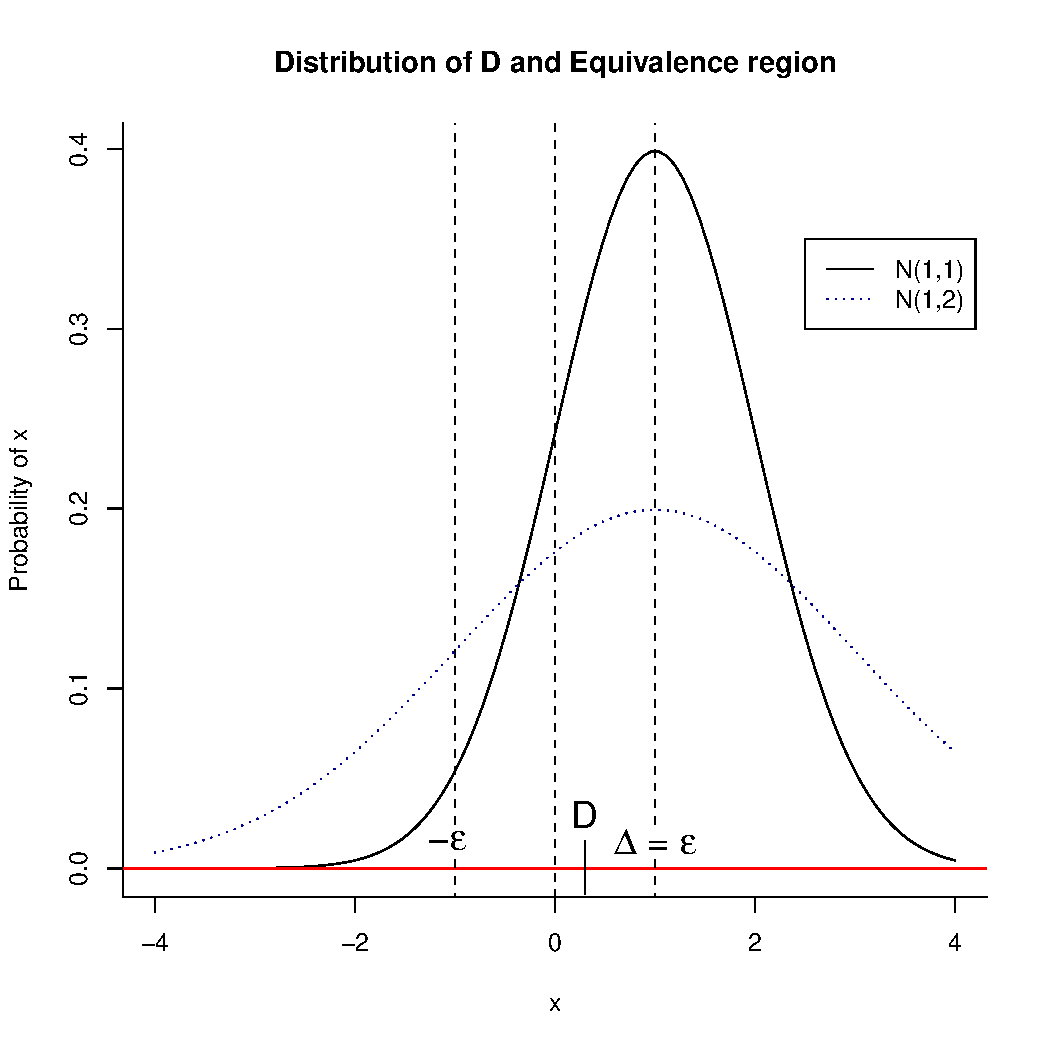
\includegraphics{DiagramNormal.pdf}
\end{center}
\caption{ The solid black line is a plot of the density function of a normal distribution with mean $\mu = \epsilon = 1$ and variance $\sigma = 1$ and the dotted blue line is a plot of the normal distribution  function for $\mu = 1$ and  $\sigma = 2$. The hash mark labelled $D$ is a hypothetical observation of a sample mean. Translating the mean of the distribution in the positive direction necessarily results in a lower likelihood of observing a sample mean inside $(-\epsilon, \epsilon)$. Increasing the standard deviation (and hence its estimator, the standard error), decreases the area beneath the curve between $\pm \epsilon$, decreasing the likelihood of measuring $D$ inside $I_\epsilon$. Finally, with mean $\epsilon$, measurements of sample mean less than $D$ in absolute value are less likely.}
\label{DiagramNormal}
\end{figure}

The distance from $D$ to the nearest endpoint of $I_\epsilon$ in units of standard errors of $D$ is given by 
\begin{eqnarray}
 K = \frac {\epsilon - |D| }{\mbox{SE}(D) },
 \end{eqnarray} 
 where SE$(D)$ is the standard error\footnote{ The standard error is an estimate of the population standard deviation. A common estimate is the sample standard deviation, given by the squared deviations from the sample mean divided by the degrees of freedom. I.e. if  $x = (x_1, \dots x_{n_x})$, then the standard error of $x$ is given by 
 $\sqrt{ \frac{1}{n_x-1} \sum_{i=1}^n (\bar{x} - x_i)^2}$ }
 of the mean difference between the $x$'s and the $y$'s. $K$ not only satisfies the conditions suggested above, but is also a measurement of a $t$-statistic, as described in Appendix \ref{Linear Regression}, meaning we can compare probability of measuring the value $K$ against the probability of  values less likely under the null. Under the null, we would expect intervals larger than $K$ to be less likely. Hence the p-value of the measurement $K$ is given by:
\begin{eqnarray}  
\label{significancelevel}
p &=&  \mathbb{P}( \mathfrak{t} \geq K),
\end{eqnarray}
where $ \mathfrak{t}$ is a Student's $t$ distributed  random variable with $n_x+n_y -2$ degrees of freedom, this probability is easy to calculate.\footnote{ If $\mathfrak{t}$ has $\nu$ degrees of freedom, $\alpha = 1 - \int_{-\infty}^K   \frac{ \Gamma (\frac{\nu+1}{2}) }{\Gamma(\frac{\nu}{2 }) } \frac{1}{\sqrt{\nu \pi}} \left( 1 + \frac{t^2}{\nu} \right) ^{-\frac{\nu+1}{2}} dt $, where $\Gamma(\cdot)$ is the Gamma function. See \cite{Intro} for more detail.}

%The factor of $2$ on the right hand side of equation \ref{significancelevel} comes from the fact that while $D$ is normal, $|D|$ is not. We need to consider both $D$ and $-D$, and hence both the distances 
%\begin{eqnarray} -K &=& \frac{-\epsilon + D}{\mbox{SE}(D) }
 %\\ & \mbox{and}& \\
%K &=& \frac{\epsilon - D}{\mbox{SE}(D) }. \end{eqnarray}
%Hence the p-value is really given by $ \alpha = \mathbb{P}(-K \geq \mathfrak{t} \  or \  \mathfrak{t} \geq K) = \mathbb{P}(-K \geq \mathfrak{t}) + \mathbb{P}( \mathfrak{t} \geq K)  $. Because the Student's $t$ distribution is symmetric about zero, this reduces to $2\cdot  \mathbb{P}( \mathfrak{t} \geq K)$, and hence equation \ref{significancelevel}.  

Rather than the method described above, for computational efficiency, an equivalent formulation of the t-test test, expressed in the language of confidence intervals, is used. We compare the limits of a level $1 - 2 \alpha$ confidence interval symmetric about $D$ to $I_\epsilon$. The level of this confidence interval is $1 - 2 \alpha$ rather than $1 - \alpha$ because it corresponds to the intersection of the rejection regions of two level $\alpha$ one sided tests. Each level $\alpha$ one sided test has a rejection region of area $\alpha$. Hence the complement of their union has area $1- 2 \alpha$. If this interval is contained completely inside $I_\epsilon$, then we have evidence of equivalence at significance level $\alpha$. In other words, we let $n = n_x + n_y -2$ and check if the following condition holds:
\begin{eqnarray} 
\label{conditionconfint}
|D| + t^{1-\alpha}_{n} \cdot \mbox{SE}(D) < \epsilon,
 \end{eqnarray}
where $t^{1-\alpha}_{n}$ is the $(1-\alpha)$-th quantile of the Student's $t$ distribution with $n$ degrees of freedom. If $D$ satisfies this condition, then we have equivalence at level $\alpha$.

A little bit of algebra will show the condition \ref{conditionconfint} is equivalent to \ref{significancelevel}: 
\begin{eqnarray}
|D| + t^{1-\alpha}_{n} \cdot SE(D) < \epsilon \\
\iff \frac{\epsilon - |D|}{\mbox{SE}(D)} > t^{1-\alpha}_{n}
\end{eqnarray}
From the definition of $t^{1-\alpha}_{n}$, if $\mathfrak{t}$ is Student's $t$ distributed with $n$ degrees of freedom,, then we know $t^{1-\alpha}_{n}$ satisfies $\mathbb{P}( \mathfrak{t}  \leq t^{1-\alpha}_{n}) = 1-\alpha$. Hence: 
\begin{eqnarray}
 \mathbb{P}\left(  \mathfrak{t} < \frac{\epsilon - |\Delta_i|}{SE(\Delta_i)} \right) &=& 1 - \alpha, 
 \\ & \mbox{and} & \\
 \mathbb{P}\left(\mathfrak{t} \geq \frac{\epsilon - |\Delta_i|}{SE(\Delta_i)}  \right) &=&  \alpha.
\end{eqnarray} 
which is equation \ref{significancelevel} with $p = \alpha$. The significance level, $\alpha$ of the test, can be thought of as the maximum p-value with which we reject the null. Hence the two formulations of the test are equivalent.






 \section{The Bootstrap Test of Equivalence}
 \label{Bootstrap}
 
 The bootstrap is a non-parametric method\footnote{That is to say: does not rely on the specification of a parametric family prior to statistical analysis.} for ascertaining the accuracy of an estimate, like the t-test. 
 
 \subsection{The Bootstrap Estimate of a Single Parameter}
 For a single parameter, the bootstrap is fairly simple. Suppose we are given  \newline $\mathbb{M} = \nolinebreak ( z_1 , \dots, z_k )$, measurements of a random variable $Z$ from an unknown distribution $F$, and we are interested in some parameter of $F$, called $\theta$, with estimator $\hat{\theta}$. Let the initial calculation of $\hat{\theta}$ be $\hat{\theta}_o$. The bootstrap algorithm is:
 \begin{enumerate}
 
 
 \item Assign probability $\frac{1}{k}$ to each $z_i$, forming the empirical probability distribution $\hat{F}$. 
 
 \item Sample from $\hat{F}$ with replacement $k$ times, obtaining a random sample, $\mathbb{M^*} =  \{z_1^* , \dots, z_k^* \} $. Calculate the same statistic, $\hat{\theta}$, using $\mathbb{M^*}$ as data. 
 
 \item Repeat Step 2  some large number, say $B$, of times, remembering each $\hat{\theta}$ along the way. Call the $i$-th calculation of $\hat{\theta}$ by $\hat{\theta}_i$.
  

 \end{enumerate}
 
This algorithm produces a bootstrapped distribution for the estimator $\hat{\theta}$ which we can use to assess the probability of measuring $\hat{\theta}_o$. Let the bootstrapped estimators be $\Theta = ( \hat{\theta}_1, \dots, \hat{\theta}_B )$. We then specify a critical region based on the bootstrap distribution. We sort $\Theta$ into ascending order. If the significance level of the test is $\alpha$, we select the $(\alpha \cdot B)$$^{th}$ and the $(1 - \alpha) \cdot B$$^{th}$ value, rounding up to the nearest integer when these are not integer values. If these two values lie inside $(-\epsilon, \epsilon)$, then we reject the null.

\subsection{The Bootstrap Test of Equivalence}

In the test of equivalence, rather than a single data set $\mathbb{M}$, our data is divided into two groups, $x$ and $y$, as above. Although the bootstrap works for any statistic which is asymptotically normally distributed, we are explicitly interested in the difference of sample means. Hence, we calculate $\bar{x}$ and $\bar{y}$, and bootstrap the estimates of both means separately. As above, we then resample $n_x$ times from $x$ and  $n_y$ times from $y$. We recompute $\bar{x}$ and $\bar{y}$ from these resamples, and then repeat this process some large number, say $B$, of times. The $i^{th}$ re-computation of $\bar{x}$ is called $\bar{x}^i$, and the $i^{th}$ re-computation of $\bar{y}$ is called $\bar{y}^i$. The bootstrap distribution of the difference: $D =\bar{x} - \bar{y}$ is obtained by considering the differences: $\Theta = ( D_1 = \bar{x}^1 - \bar{y}^1, \dots, D_B = \bar{x}^B - \bar{y}^B )$

The null hypothesis is:
\[ \Delta \notin I_\epsilon \]
In parallel with the t-test test of equivalence above, if $D \notin I_\epsilon$, we cannot reject the null. If $D \in  I_\epsilon$, we ask how likely we are to measure differences as or less likely than $\epsilon$. As we have made no assumptions about the distribution of $D$, we have no reason to suppose any element of $I_\epsilon$ is more likely than any other.  Hence, we simply measure the proportion of the bootstrap distribution which violates the null and compare it to the significance level $\alpha$.  We sort the values of $\Theta$ in ascending order. We call the $\lceil \alpha \cdot B \rceil^{th}$ value $D_{lo}$ and the $ \lceil (1 -  \alpha)\cdot B \rceil$ $^{th}$ value\footnote{The notation $\lceil x \rceil$, where $x$ is a real number, refers to the least integer greater than $x$. } $D_{hi}$. Then, if the interval $(D_{lo}, D_{hi})$ is contained in $I_\epsilon$, we declare equivalence at significance level $\alpha$.  This is exactly the percentile confidence interval described in \cite{BootstrapBook} . 
 



\chapter{Application to the Analysis of Microarray Data}

\label{Analysis of Microarray Data}

The workhorse of microarray data analysis is the linear model. However, microarrays have a few nonstandard features which complicate the analysis.

 
 In the microarray context, our hypothesis is about a statistic, $\Delta$, which measures the log ratio of gene expression between two groups of sources. If there is no difference, $\Delta$ = 0. Let $D$ be an estimator for $\Delta$. In the microarray context, the test of equivalence holds:
 \begin{eqnarray} 
 H_0: &  \Delta  \notin & (-\epsilon, \epsilon)   \nonumber \\
 & \mbox{versus}& \label{ToEQ}\\
 H_1: &  \Delta  \in &  (-\epsilon, \epsilon) \nonumber
 \end{eqnarray}
Here $\epsilon$ is some small number chosen by the scientist for substantive, scientific reasons. For instance, it is theorized that there are some genes necessary to the normal functioning of cells - called housekeeping genes because the functions for which they are responsible are so rudimentary - which should be expressed uniformly across phenotypes within species. For the purpose of detecting housekeeping genes, one might choose a relatively small epsilon. If we are looking for genes equivalently expressed across species, we might want a larger $\epsilon$ to allow for inter-species differences which might adjust gene expression levels \cite{QiuandCui}.

Microarray analysis often involves (as in \cite{adjaye}, \cite{Renn} and \cite{rodriguez}) fitting a linear model to produce estimates of relative gene expression level. As such,  appendix \ref{Linear Regression} covers a common method, least squared error linear regression, along with the construction of Student's $t$ statistic employed in the two one sided $t$-test. 

The first thing of note when analyzing microarray data is the sheer number of data sets. Renn et al [2008] employed forty microarrays, each of which had $6,400$ features. Hence in its analysis, one must run linear regressions on $6,400$ data sets of forty data points to test each of $6,400$ hypothesis. These numbers require significant amount of computational resources.

 As described in Appendix \ref{Linear Regression}, a linear model describes the relationship between response variables and a set of explanatory variables. The response variables in the microarray context are measurements of ratios of intensity between two dyes for a given feature on a given array. For ease of comparison, analysts typically employ the log ratio of intensity levels. 
 
 In microarray analysis, the explanatory variables are discrete, specifying simply the presence or absence of a source\footnote{Tissues compared on microarrays are referred to as sources, in general.} on a given array. The explanatory variables are written down in  the design matrix. In this context, each row of the design matrix corresponds to an array, while each column corresponds to a source. If a source, say the k$^{th}$ one, is dyed with Cyanine 3 and hybridized on the i$^{th}$ array, a ``1" is written down in the ($i,k)$$^{th}$ position. If the same individual is dyed with Cyanine 5 instead, a ``-1" would be recorded in the $(i,k)$$^{th}$ position. Otherwise, a zero is written down. For example these are two plausible rows of a design matrix.
 
 \begin{eqnarray}\begin{array}{ r | r r r r r r r} 
 	\label{fig: RowsDesign}
 
    &  \dots & k -1 &k &k+1 & k+2 & k+3 & \dots \\ \hline		
i  &\dots & 0 & 1 & 0 & -1 & 0 &\dots\\
i+1 & \dots &  0 & -1 & 1 & 0 & 0 &\dots \\

\end{array}
\end{eqnarray}
 
 From \ref{fig: RowsDesign} we can read that on the $i^{th}$ array, the $k^{th}$ individual (in Cyanine 3) was compared to the $(k+2) ^{th}$ individual (in Cyanine 5). 
 
 Given the the design matrix, $X$, and the response variables, a vector $Y$, a linear model is fitted, producing estimated expression coefficients\footnote{Each feature has an associated vector of estimated coefficients, fitted values, and residuals. Each of these vectors has one entry for each source.} $\hat{\beta}$, fitted values $\hat{Y}$ and residuals $\mathbf{r}$. In least squared error regression, we assume the random error of each measurement is independent from all other measurements, and that this random error has constant variance and mean zero.  Until this point - that is up until section \ref{Distributional Results} of Appendix \ref{Linear Regression} - the least squared error linear regression relies on no distribution specific assumptions. At this point, one can choose to assume normal error and apply the TOST test of equivalence, or instead make the much looser assumption that the difference statistic is asymptotically normal\footnote{A statistic is asymptotically normal if and only if, as the sample size grows arbitrarily large, the statistic's distribution becomes arbitrarily close to the normal distribution. See Chapter 7.2 of \cite{Intro} for more information. The most common example of an asymptotically normal distribution is the sample mean (by the Central Limit Theorem).}, and apply the Bootstrap.


\section{ Contrasts }

Once the the linear model has been fitted, we are left with $\hat{\beta}$, the vector of relative log gene expression level sources and some baseline reference source. We want to compute the difference in mean expression levels between two different phenotypes - subgroups of our sample grouped by distinctive physical or behavioral characteristics. To this end, one introduces a contrast vector: 
\begin{eqnarray} c = \left(\begin{array}{c} 
 c_1 \\ c_2 \\ \vdots \\ c_n
 \end{array}\right)  
 \end{eqnarray}
such that  $\sum_{i=1}^n c_i = 0$. Each entry of $c$ corresponds to a source in the experiment.  In microarray analysis, $c$ is chosen in such a way so that $ c^t \beta = \sum_{i=1}^n c_i \beta_i$ is the difference of average log gene expression levels between two phenotypes; i.e. $c^t \beta = \mu_1 - \mu_2$, where $\mu_1$ and $\mu_2$ are mean relative expression levels in groups 1 and 2,  as compared to reference. For example, suppose we have four sources, divided up into two phenotypes. Suppose sources one and two are in one group and sources three and four are in the other. Let $\hat{\beta}_1, \hat{\beta_2}, \hat{\beta_3}$ and $\hat{\beta_4}$ be the corresponding estimated expression levels. Then an appropriate choice of contrast vector would be $c = (0.5, 0.5, -0.5, -0.5)$. When we take the inner product,
 \[ 
 c^t \hat{\beta} = \frac{\hat{\beta}_1 + \hat{\beta_2}}{2} - \frac{\hat{\beta_3} +\hat{\beta_4} }{2},
  \]
we find that $c^t \hat{\beta}$ is the difference in  estimated mean expression levels between the two groups. 



\section{A Very Simple Example}

To make this discussion more concrete, suppose, once again, we are comparing Lemurs from phenotype A to Lemurs from species B. Imagine we have two sources from each species, Lemurs $A_1$ and $A_2$ and $B_1$ and $B_2$, and only two features on each array. say Gene $e$ and Gene $d$.

First we design an experiment. 
\begin{figure}[h!]
\begin{eqnarray*}
\xymatrix{  
A_1 \ar[r]^1 & A_2  \ar[d]^2 \\
B_1  \ar[u]^4  & B_2 \ar[l]_3
}
\end{eqnarray*}
\caption{This figure represents the experimental design. Arrows represent arrays and alpha-numerals represent sources.  Connecting two alpha-numerals with an arrow indicates the corresponding sources were compared on the array whose index is shown adjacent to the arrow. A source positioned at the head of an arrow indicates it was dyed, on the corresponding array, with Cyanine 3, and at the tail with Cyanine 5.}
\label{SimpleExample}
\end{figure}

 
We can read the design matrix directly from figure \ref{SimpleExample}. One might think the design matrix would be:

\begin{eqnarray*}
  \left( \begin{array}{r r r r} 
  -1 & 1 & 0 & 0 \\
 0  & -1 & 1 & 0 \\
 0 & 0 &  -1 & 1 \\
 1 & 0 & 0 & -1 \\ 
\end{array} \right)
\end{eqnarray*}

This would be correct, except microarrays always compare two different sources. That is they do not measure absolute gene expression levels, but rather gene expression levels relative to some source set as reference. The estimated expression coefficients represent lof ``fold change"-- e.g. this gene is expressed three times as much in source $A_2$ as in the reference source, whichever that may be. Encoding the design matrix as above would imply that we could obtain absolute measurements for every gene expression level. Not only is this design experimentally impossible, but it also leads to a singular design matrix -- a big problem for linear regression. 
	To avoid these problems, we set one lemur as reference, say lemur $A_1$, whose relative gene expression level is set to zero. Rather than keep track of him throughout the experiment, we simply delete the column corresponding to lemur $A_1$ from the design matrix, yielding:

\begin{eqnarray}
X =  \left( \begin{array}{ r r  r} 
   1 & 0 & 0 \\
  -1 & 1 & 0 \\
  0 &  -1 & 1 \\
 0 & 0 & -1 \\ 
\end{array} \right)
\end{eqnarray}

The design is important. A faulty design will deny the analyst the ability to compare expression ratios between all the sources in the experiment. Every source should appear on at least two arrays, once in Cyanine 3 and once in Cyanine 5, to avoid dye bias, and each source should appear in such a way so that the gene expression of every source can be compared to all other sources. 

Suppose we measured the following fluorescence ratios for two genes on the arrays\footnote{In most papers these would be on a log$_2$ scale, but for now, these have been presented in the original scale}:

\begin{eqnarray}
\label{table: fakemicroarray}
\begin{tabular}{c | c c c c}
             & Array 1 & Array 2 & Array 3 & Array 4 \\ \hline
Feature d  & 1.78 & 5.46 & 1.83 & 2.20\\
Feature e  & 0.92 & 0.95 & 0.85 & 0.42   \\
\end{tabular}
\end{eqnarray}

In this design, we can compare any individual's fluorescence levels to any other's. One can deduce this from figure \ref{SimpleExample}. On the graph, there is a path| i.e. a chain of comparisons from any source to any other. Hence because comparisons of gene expression levels are transitive, we can compare any source to any other.

The rows of the table \ref{table: fakemicroarray} make up the response variables $Y$ in two separate experiments. They share a design matrix, because the experimental design remains unchanged as the feature under consideration varies.

Let us compute log$_2$ relative gene expression levels using the values from \ref{table: fakemicroarray}, as described in detail above.  

First, on conversion to base 2 logarithms, \ref{table: fakemicroarray} becomes:

\begin{eqnarray}
\label{table: logfakemicroarray}
\begin{tabular}{c | c c c c}
             & Array 1 & Array 2 & Array 3 & Array 4 \\ \hline
Feature d  & 0.83 & 2.44 & 0.87 & 1.13  \\
Feature e  & -0.11 & -0.07 & -0.23 & -1.24   \\
\end{tabular}
\end{eqnarray}

The estimated expression of Gene $d$ and Gene $e$  as compared to the reference in the three, non-reference lemurs in the experiment is given by an application of \ref{CoeffEst}:

\[ \hat{\beta}_d = (X^t X)^{-1} X^t Y_d =  \left( -0.49\, ,\,0.63\, , \, 0.19  \right) \]
\[ \hat{\beta}_e = (X^t X)^{-1} X^t Y_e = \left(0.30 \, ,\, 0.64 \, , \,  0.827 \right) \]

 
A natural contrast vector for this experiment is $c = (1/2,\, -1/2,\, -1/2)$, which would specify that $A_2$ is in one group of two with the reference source, $A_1$, and that $B_1$ and $B_2$ are in the other of two. There is only one positive entry because the source corresponding to the other positive entry is the reference, and would be multiplied by zero anyway. 

With this contrast vector, we have:
\[ c^t\hat{\beta}_d  =  -0.6554229\]
and
\[ c^t\hat{\beta}_e  =  -0.5837189\]

This sample size is so small that running the tests of equivalence on them is not really worthwhile. Both the TOST and Bootstrap test of equivalence are described in application to microarray data in what follows.

\section{The t-Test and Bootstrap for Microarray Data}

Both the t-test and the bootstrap tests of equivalence can be formulated in terms of contrasts. In both tests, the estimator for $\Delta = c^t \beta$ is $D = c^t \hat{\beta}$, where $c$ is a contrast vector, $\beta$ is a vector of true gene expression levels, and $\hat{\beta}$ is it's estimate.  The hypothesis test is unchanged:
 
 \begin{eqnarray} 
 H_0: &  \Delta  \notin & (-\epsilon, \epsilon)   \nonumber \\
 & \mbox{versus}& \label{ToEQ}\\
 H_1: &  \Delta  \in &  (-\epsilon, \epsilon) \nonumber
 \end{eqnarray}
 
 If $|D| \geq \epsilon$, neither test can reject the null. Otherwise, the procedures described in the following subsections are carried out.
 
 \subsection{t Test of Equivalence for Microarrays}

The TOST test for microarray data relies on the distributional results from \ref{Distributional Results} Specifically:

\begin{eqnarray}
 \label{eqn: hatbeta}
 \hat{\beta} \thicksim N(\beta, \,\sigma^2 (X^tX)^{-1}).
  \end{eqnarray}

From \ref{eqn: hatbeta}, we can deduce, by brief application of \ref{Cov} and  \ref{Mean},  the distribution of  $c^t \hat{\beta}$,
\begin{eqnarray}
\label{c^t beta}
c^t\hat{\beta} \thicksim N( c^t \beta, \,\sigma^2 c^t (X^tX)^{-1}c).
\end{eqnarray}
Hence we can construct for $c^t \hat{\beta}$ a $t$-statistic, which we can use in a $t$-test:
\begin{eqnarray}
t = \frac{c^t  \hat{\beta} - c^t  \beta }{ s \sqrt{ c^t (X^tX)^{-1}c} },
\end{eqnarray}
where $s$ is the residual standard error. $t$ has the Student's $t$ distribution with degrees of freedom equal to $df$, the difference in the number of explanatory and response variables. 



Recall that the TOST rejects the null hypothesis at level $\alpha$ when the p-value $ \mathbb{P}(\mathfrak{t} \geq K) < \alpha$, where $\mathfrak{t}$ is Student's $t$ distributed with the $df$ degrees if freedom, and $K $ is given by 
\begin{eqnarray}
 K = \frac {\epsilon - |D| }{\mbox{SE}(D) }.
 \end{eqnarray} 
 Equivalently, the test rejects $H_0$ if
 \[
|D| + t^{1-\alpha}_{df} \cdot SE(D) < \epsilon
\]
In the microarray context, $\mbox{SE}(D)$ is given by $s \sqrt{ c^t (X^tX)^{-1}c} $, and $D = c^t \hat{\beta}$. Hence, we reject the null hypothesis of non-equivalence with level $\alpha$ when 
\[p =   \mathbb{P}( \mathfrak{t} \geq K) < \alpha,\]
where $K$ is given by:
\[ K = \frac {\epsilon - |c^t \hat{\beta}| }{ s \sqrt{ c^t (X^tX)^{-1}c}  }, \]
and $\mathfrak{t}$ is Student's $t$ distributed with $df$ degrees of freedom.


\subsection{The Bootstrap for Microarray Data}
 
In the microarray context, the set of data to be bootstrapped - $\mathbb{M}$ - is the set of estimated gene expression levels (in log scale) for a given feature, including the estimated gene expression of the reference animal, a zero. Explicitly, $$ \mathbb{M} = \left(0, \hat{\beta}_1, \hat{\beta}_2, \dots, \hat{\beta}_n \right)$$ If $D \in  (-\epsilon, \epsilon)$, then we employ the bootstrap.  We divide $\mathbb{M}$ into groups as indicated by the contrast vector, and then resample from each group of entries seperately. In this way, we construct the bootstrap distribution: $$\Theta = \left( c^t \hat{\beta}^1, \dots, c^t  \hat{\beta}^B \right),$$ where each $c^t \hat{\beta}^i$ is formed by sampling from $\mathbb{M}$, as described in section \ref{Bootstrap}. We sort $\Theta$ into ascending order\footnote{The notation $x^{(i)}$ in this context represents the $i$-th ordered element of all the $x$'s}: $$\Theta^\circ = \left(c^t \hat{\beta}^{(1)}, \dots, c^t \hat{\beta}^{(B)}\right).$$ Given $\Theta^\circ$ and a given significance level $\alpha$, we compute $n_{1} = \lceil \alpha \cdot B \rceil$ and $n_2 = \lceil (1 - \alpha) \cdot B \rceil$ and compare the interval $I_B = ( c^t\hat{\beta}^{(n_1)},  c^t\hat{\beta}^{(n_2)})$ to  $I_\epsilon = (-\epsilon,\  \epsilon)$. If $I_B \subset I_\epsilon$, we reject the null hypothesis at level $\alpha$.
 

\chapter{Analysis of Tests}
\label{Analysis}

Both tests as described in sections \ref{TOST} and \ref{Bootstrap} are applied to several artificial data sets in order to assess each test's \emph{power} | that is, the probability that each test rejects a false null hypothesis. In more formal language, the power of a test is given by $\Pi = \mathbb{P}(\mbox{Reject}\  H_o \  | \ H_1 )$.

Both tests are assessed by generating data sets for which $\Delta$, the true difference, is less than $\epsilon$. Recall that the null hypothesis for these tests is:
\begin{eqnarray}
H_o: \Delta \notin (-\epsilon, \  \epsilon)
\end{eqnarray}
In this assessment $\Delta$ is set to several different values inside the interval $(-\epsilon, \  \epsilon)$, so that both tests should reject the null and declare equivalence for every random sample considered. The data sets are constructed by specifying two vectors of length $n$, $x$ and $y$, with the same distribution. A standard normal data set and a Student's $t$ data set with six degrees of freedom were tested.

The more efficient method described in section \ref{TOST} is used here. That is, given $m$ random samples, each with estimated difference $D_i$, we check to see if the random samples satisfy:

\begin{eqnarray} 
\label{confint}
|D_i| + t^{1-\alpha}_{n-2} \cdot SE(D_i) < \epsilon
 \end{eqnarray}

The proportion of $D_i$ satisfying condition \ref{confint} out of all $m$ random samples gives a measure of the power of the t-test.

The measure of power is similar for the Bootstrap. The Bootstrap test of equivalence as described in section \ref{Bootstrap} is run on $m$ random samples. The proportion of random samples declared equivalent out of the total number ($m$) of random samples gives the power of the Bootstrap.

With normally distributed data, we expect the t-test to perform better. In the Student's $t$ distributed data set we expect the Bootstrap to perform better than the $t$ test. To test these hypotheses, power computations for every sample size between $n= 6$ and $n = 45$ were carried out, producing the figures below. $\epsilon$  is set to one. Each power computation involved 1,000 samples, each of length $2n$, divided into two groups. For each sample size, 1,000 bootstrap repetitions were carried out.
\pagebreak

\begin{figure}[h!]
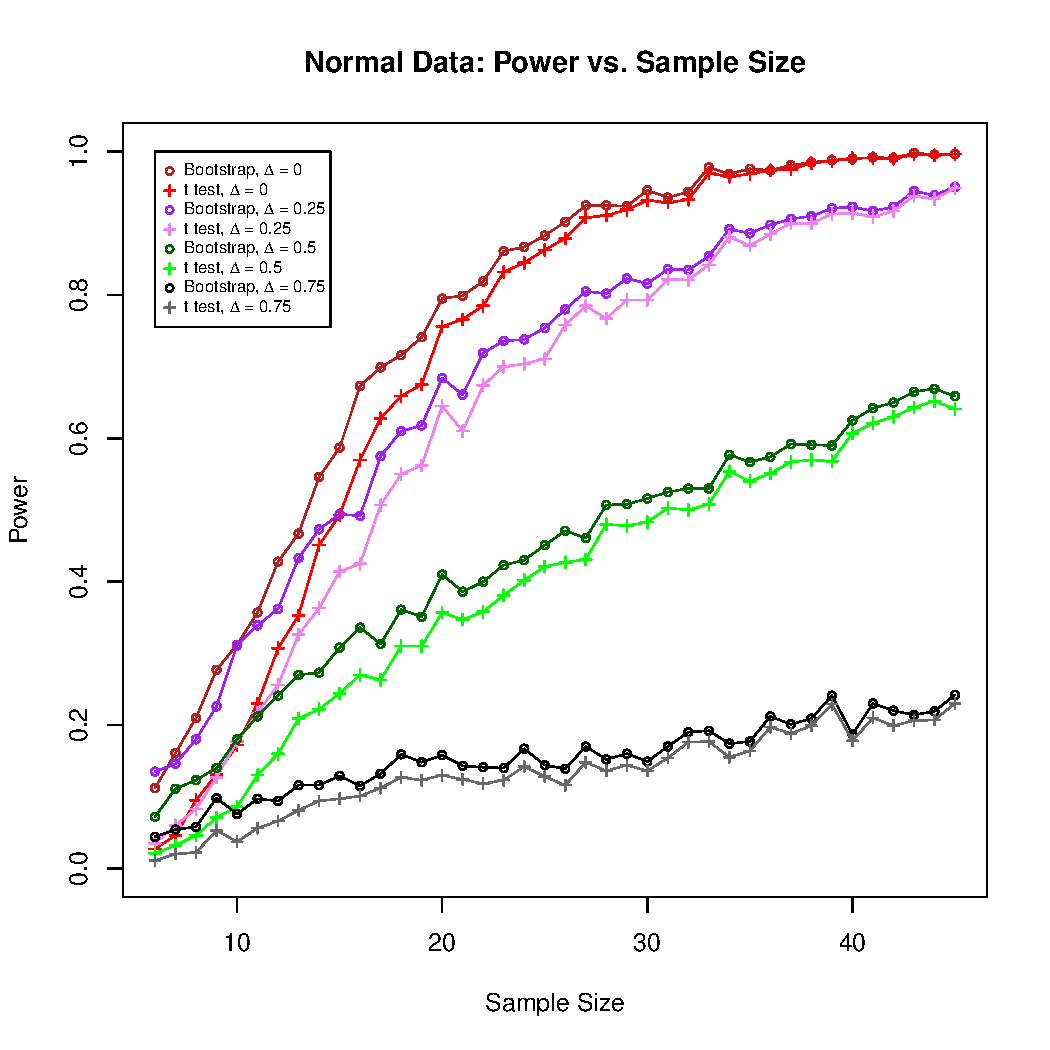
\includegraphics{NormalPowerEpsilon.pdf}
\caption{Normal data was divided into two groups, one with mean $0$ and the other with mean $\Delta$ as shown in the legend. Both groups have variance one. The bootstrap is represented with circles, and the t-test with crosses. Both tests reject the null if the 97.5\% confidence interval about the difference of means is not contained in $(-1,1)$}
\label{NormalPowerEpsilon}
\end{figure}

\pagebreak

\begin{figure}[h!]

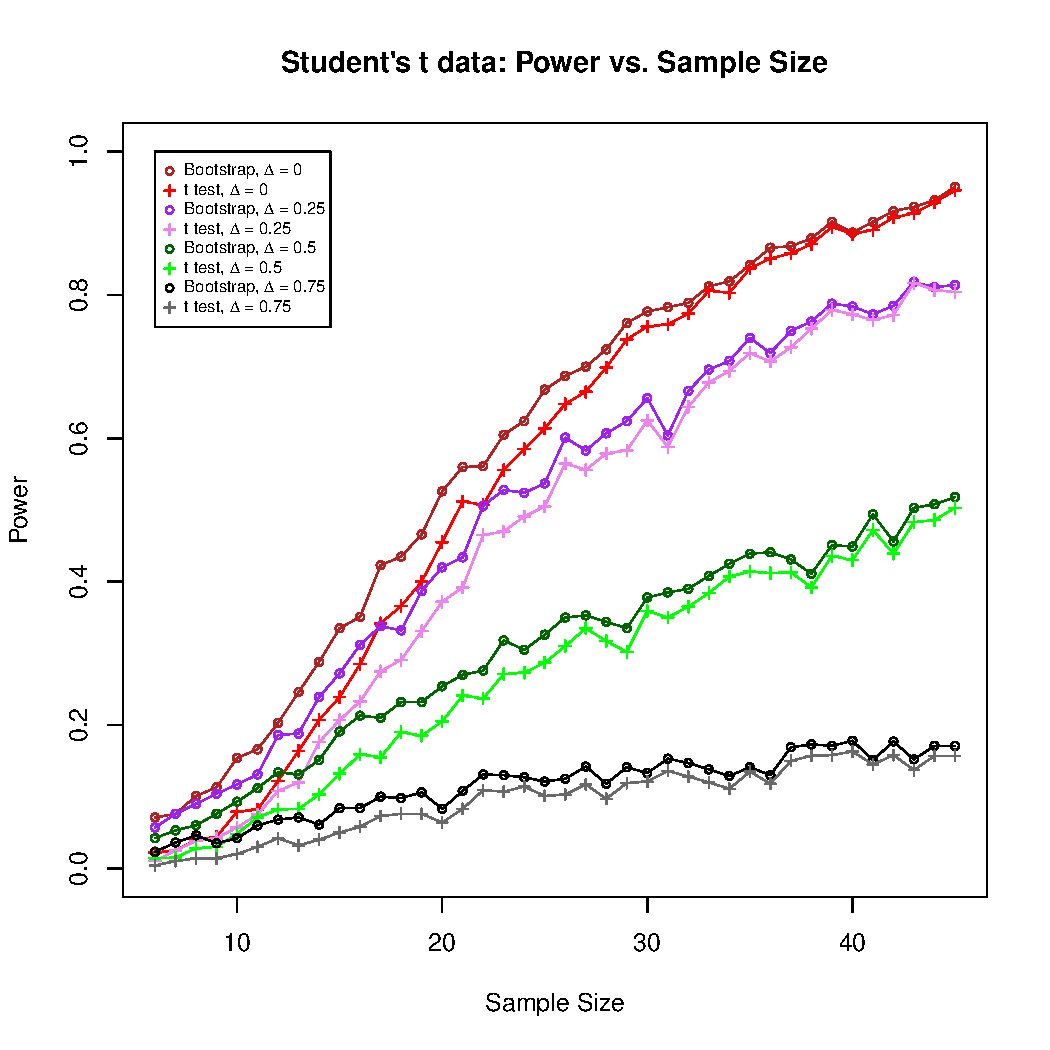
\includegraphics{Student'sTPowerEpsilon.pdf}

\caption{Student's $t$ data with six degrees of freedom was divided into two groups, one linearly shifted $\Delta$ away from zero, as shown in the legend. The bootstrap is represented with circles, and the t-test with crosses. Both tests reject the null if the 97.5\% confidence interval about the difference of means is not contained in $(-1, 1)$}
\end{figure}

\pagebreak

Against expectations, the bootstrap out-performs the t-test for normal data until the two reach agreement with high sample sizes (see figure \ref{NormalPowerEpsilon}). The difference is most pronounced for very small sample sizes and values of $D$ firmly inside the interval $( -\epsilon, \epsilon)$. As $D$ grows closer to $\epsilon$, the power of both tests decreases. The difference in powers also decreases as $D$ approaches $\epsilon$, as evidenced by their near-equally dismal power at $D = 0.75$. For normal data the average difference in power | that is the sample average of $\Pi_B - \Pi_{\mbox{\tiny{t-test}}}$ over sample sizes between six and twenty and twenty and forty five is given by:

\begin{eqnarray}
\label{table: normaldataPowerdifference}
\begin{tabular}{r | r  r r}
             & D = 0 & D = 0.25 & D = 0.5 \\ \hline
n $\leq$ 20  & 0.0813 & 0.077 & 0.0575  \\
n $> 20$ & 0.0061 & 0.0136 & 0.02475   \\
\end{tabular}
\end{eqnarray}


If the computing power is available and the data is normal there is evidently a clear advantage to using the bootstrap over the t-test, especially in circumstances with small data sets.

%\pagebreak

When applied to Student's $t$ distributed data, the performance of both tests decreased. The bootstrap continued to have greater power than the t-test, but by a smaller margin. For Student's $t$ data, the sample average of $\Pi_B - \Pi_{\mbox{\tiny{t-test}}}$ over sample sizes between six and twenty and then twenty and forty five is given by:

\begin{eqnarray}
\label{table: studentstdataPowerdifference}
\begin{tabular}{r | r  r r}
             & D = 0 & D = 0.25 & D = 0.5 \\ \hline
n $\leq$ 20  & 0.0663 & 0.05475 & 0.0435  \\
n $> 20$ & 0.0144 &0.01775 & 0.023   \\
\end{tabular}
\end{eqnarray}

Once again, there is a clear advantage to using the bootstrap over the t-test, but it is  slightly less pronounced as with normal data.

These results are unexpected to say the least. We would expect the satisfaction of the normal assumptions upon which the t-test relies to grant it advantage over the bootstrap. That it does not is cause for concern, and possibly an indication of an error in methodology. However, at the time of this writing, none could be found.








\chapter{Conclusion}
Two tests of equivalence were described in theory and in application to microarray data analysis. Code to carry out the application of both tests can be found in Appendix \ref{Code}. There is quite a bit left to be done. The greater power of the bootstrap when applied to normal data found in chapter \ref{Analysis} runs counter to common sense. It would seem to imply that it is better to ignore clear evidence that data is normal than to take this information into account (for small sample sizes).

 Possible explanations for the this surprising result are an error in the R-script use to run the tests, an error in the generation of data, or that the common sense the result contradicts is simply wrong. The R function used to generate data is well tested, leaving code error as the remaining flaw. With more time, an alternative execution of both tests should be implemented so as to corroborate results, and the code of both implementations should be carefully inspected. Additionally, perhaps there is a theoretical argument for the superiority of the Bootstrap over the t-test in the one-sided case with normal data. In any event, further research is needed.
 
It would be appropriate to apply these tests to the analysis of data from an experiment designed to produce equivalent data sets. For example, Susan C. P. Renn's laboratory compiled a data set in which every sample on the microarray came from the same source, at roughly the same time. We can reasonably assert that every sample is equivalent to the reference\footnote{If a tissue is not equivalent to itself, then the term has no meaning}, and hence use this data set to assess the power of the two tests of equivalence.

Finally, a better critical interval could be developed. It is not at all clear that the interval $I_\epsilon = (-\epsilon, \epsilon)$ is the best one for these purposes. It is simply the simplest and most intuitive. There may be good reason to use a smaller interval - to reduce the probability of type II error - or a larger one to increase power. 

\appendix
     \chapter{ Linear Regression }
\label{Linear Regression}
Linear regression is designed to analyze experiments in which each of $n$ responses is supposed to be a consequence of a set of $m$ explanatory variables. We usually suppose that there are at least as many responses as explanatory variables, i.e. $n >m$, otherwise we have fewer equations than variables and the system has no unique solution. In fact, if it is the case that there are fewer response variables than explanatory variables, it would behoove the statistician to advise the scientist to cary out more runs of the experiment. The collection of responses is written down in an $n \times 1$ vector called $Y$, and the explanatory variables are written down in an $n \times m$ matrix, $X$, called the design matrix. As this is a linear model, we suppose $X$ and $Y$ are linearly related to each other, and subject to random error, $\delta$. $X$ is referred to as the design matrix. One might express the supposed relationship between $X$ and $Y$ as follows: 
\begin{eqnarray} y_i = \beta_1 + \beta_2 x_{i2} + \beta_3x_{i3} + \dots + \beta_m x_{im} + \delta_i  \quad : \quad i = 1, \dots , n \;.\label{LinearModel} \end{eqnarray} 
The $\beta_j$ are unknown quantities referred to as the ``regression coefficients.'' Note that in order to accommodate an intercept term  $x_{i1}$ is assumed to be unity for $i = 1, \dots, n$. It will simplify matters down the road to use matrix notation:\footnote{for a review of matrices and linear algebra, see \cite{linear}. I will use results and definitions from this text liberally.} \begin{eqnarray} Y = X \, \beta + \delta \,, \label{MatrixLM} \end{eqnarray}
where $\beta$ is the $m \times 1$ vector of $\beta_j$'s. In the standard linear model, one assumes that error is independently, identically normally distributed with variance $\sigma^2$: 
\begin{eqnarray}  \delta \thicksim N( \mathbb{O} \;,\; \mathbb{I} \, \sigma^2) \,, \label{MatrixError}\end{eqnarray}
where $\mathbb{I}$ is the identity matrix in $\mathbb{R}^n $ and $ N(\mathbb{O} \,,\, \mathbb{I} \, \sigma^2)$ is the multivariate normal distribution with mean equal to the zero vector and covariance matrix  $ \mathbb{I} \, \sigma^2$.

The end goal of carrying out a linear regression is to obtain an estimator for $\beta$, call it $\hat{\beta}$. $\hat{\beta}$ is the $m$-dimensional analogue to the slope of the line which best fits the data. The basic idea is to minimize the distance between any data point and the ``line;" that is to minimize the magnitude of the \emph{residuals}: $\mathbf{r} = Y-\hat{\beta} \,X$. The residuals vector is given by solving \ref{MatrixLM} for $\delta$. 

We will later show that $X \, \hat{\beta}$ is an unbiased\footnote{ An estimator $\hat{\theta}$ of $\theta$ is unbiased if $\mathbb{E}(\hat{\theta}) = \theta$} estimator for $Y$. For this reason, we say: \begin{eqnarray} \label{fitted} \hat{Y} = X \hat{\beta}\;, \end{eqnarray}and call the entries of $\hat{Y}$ ``fitted values." The residuals are a measure of how close the fitted values are to the actual values of $Y$.

There are a number of methods by which the minimization of residuals can be done. Ordinary least squared error regression is described here. The sum of the squared residuals, \begin{eqnarray} \label{squaredresidual} \mathbf{r}^t\mathbf{r}=(Y-\hat{\beta} \,X)^t(Y-\hat{\beta} \,X) \,,\end{eqnarray} is minimized with respect to $\hat{\beta}$. 

In algebraic terms, choosing $\hat{\beta}$ which minimizes the sum of squared residuals is the same as choosing the vector in the column space of $X$ closest to $Y$ \cite{Regression}.  If one were to draw a cartoon of the situation, imagine we are in three space, and that the columns of $X$ span the $x$-$y$ plane. $Y$ floats somewhere above the plane. $X \hat{\beta}$ is directly below $Y$. It should be clear to see that the vector $Y - X \hat{\beta}$ is perpendicular to every vector in the column space of $X$. This yields the condition: 
$ X^t (Y - X\hat{\beta}) = \mathbb{O}\,. $ 
Solving for $\hat{\beta}$ :
\[  X^t Y = X^t X \hat{\beta} \,.\]
So long as $X$ (an $n \times m$ matrix) has rank $m$, we can left multiply by $(X^t X)^{-1}\,,$ obtaining:
\begin{eqnarray} \label{CoeffEst} \hat{\beta} = (X^t X)^{-1} X^t Y\,,\end{eqnarray}
leading to fitted values 
\begin{eqnarray} \label{Fitted}
 \hat{Y} =  X (X^t X)^{-1} X^t Y \,,
 \end{eqnarray}
 and residuals: 
\begin{eqnarray} \label{residual}
 \mathbf{r} = Y - X (X^t X)^{-1} X^t Y = (\mathbb{I} - X (X^t X)^{-1} X^t )Y\,. 
 \end{eqnarray}
 Additionally, we can compute the standard error of the residuals, $s$:
 \begin{eqnarray} 
 \label{s2} s = \sqrt{ \frac{\mathbf{r}^t\mathbf{r}}{n-m} }\,,
 \end{eqnarray}  
 
Let us examine $\hat{Y}$, $\hat{\beta}$ and $\mathbf{r}$ a little more closely. $\hat{\beta}$ is the vector of linear combinations of the columns of $X$ which is closest to $Y$, and $\hat{Y}$ is in the column space of $X$. Recall that $ \hat{Y} =  X (X^t X)^{-1} X^t Y \,.$  On this ground I assert that the operator $ X (X^t X)^{-1} X^t$, let it be called $\mathbb{H}$, is an operator which picks out the element in the column space of $X$ closest to the input vector from $\mathbb{R}^n$; that is, if each $X_i$ is the $i^{th}$ column of $X$, then \[\mathbb{H}:\mathbb{R}^n \longrightarrow \mbox{Span}(X_1, \dots, X_m)\,,\]  is a projection operator into $\mbox{Span}(X_1, \dots, X_m) $, an $m$-dimensional subspace of $\mathbb{R}^n$. 
%must read linear algebra book to back these kind of statements up.

The proof of the above assertion is easy. First, the proposition that the matrix representation of any linear operator maps into its column space follows directly from the definition of matrix multiplication. Let $A$ be an $n \times m$ matrix and $B$ be an $m \times p$ matrix. Let  $A_{ij}$ be the $ij^{th}$ entry of the matrix $A$, and likewise for $B_{ij}$ and $(AB)_{ij}$. Then matrix multiplication is defined by:
 \[ (AB)_{ij} = \displaystyle\sum_{k=1}^n A_{ik} \, B_{kj} \, ; \qquad 1 \leq i \leq m \,,\, 1\leq j \leq p \,.\]
In particular, $\beta$ is $m \times 1$ and $X$ is $n \times m$. Hence $X\beta$ is $n \times 1$ and: \begin{eqnarray} (X \, \beta)_{i} &=& \displaystyle\sum_{k=1}^m X_{ik} \, \beta_{k}  ; \qquad 1 \leq i \leq m  \end{eqnarray}

\begin{equation}  \Rightarrow X \beta = \left( \begin{array}{c} \displaystyle\sum_{k=1}^m X_{1k} \, \beta_{k} \\ \vdots \\ \displaystyle\sum_{k=1}^m X_{mk} \, \beta_{k}  \end{array}\right) =  \displaystyle\sum_{k=1}^m \left( \begin{array}{c} X_{1k} \,  \\ \vdots \\  X_{mk} \end{array}\right) \beta_{k}, \end{equation}
which is a linear combination of the columns of X, proving the assertion.

Let us specify what it means to say that $H$ is a projection operator. Given a subspace $\mathbb{U}$ of a vector space $\mathbb{V}$, there is another subspace $\mathbb{W}$ such that any vector $V \in \mathbb{V}$ can be written as the sum of a vector $U$ in $\mathbb{U}$ and a vector $W$ in $\mathbb{W}$.  A projection operator \[ \mathfrak{p} :  \mathbb{V} \rightarrow \mathbb{V} \] can be characterized fundamentally by the property that given $V \in \mathbb{V}$, 
 \[ \mathfrak{p}(V) = U\,,\] 
 where  $V = U + W\,,$ and of course $U \in \mathbb{U} \;, \; W \in \mathbb{W}$. When this is the case, we say $\mathfrak{p}$ is a projection on $\mathbb{U}$ along $\mathbb{W}$. Consequently, $ \mathfrak{p}(U) = U$, and hence $ \mathfrak{p}^2(U + W) =  \mathfrak{p}(U) = U \,$. In fact,
 \begin{eqnarray} \label{projectioncondition}  \mathfrak{p}^2 =  \mathfrak{p}\end{eqnarray}
 is not only necessary but also a sufficient condition to prove that $ \mathfrak{p}$ is a projection. 
 
 We have already shown that \ref{projectioncondition} is necessary given that $\mathfrak{p}$ is a projection. Now let us show that it is sufficient:
 
 Suppose $\mathfrak{p}^2 =  \mathfrak{p}$ for some linear operator, $\mathfrak{p} : \mathbb{V} \rightarrow \mathbb{V}$. Then I propose that there exists subspaces $\mathbb{U}$ and $\mathbb{W}$ such that any vector $V$ in $\mathbb{V}$ can be written as the sum of $U \in \mathbb{U}$ and $W \in \mathbb{W}$, and $\mathfrak{p}(V) = U$.
 
 Let us note a few facts at our finger tips:  Condition \ref{projectioncondition} implies that the range of $\mathfrak{p}$ is invariant under transformation by $\mathfrak{p}$. Further the null space, or kernel, of $\mathfrak{p}$ is, by definition, always mapped to the zero vector. Both the range and the kernel, let us denote them by $R(\mathfrak{p})$ and $N(\mathfrak{p})$ respectively, are subspaces\footnote{They are clearly subsets of $\mathbb{V}$. The vector space axioms, found on page six of \cite{linear} are easily verified by the reader.} of the vector space $\mathbb{V}$, and finally, $\mathbb{V} = N(\mathfrak{p})  \oplus R(\mathfrak{p})$ that is, $\mathbb{V}$ is the direct sum of the range and null space of $\mathfrak{p}$. Taking this all together, we have that $\mathfrak{p}$ is a projection on its range along its null space, and hence $\mathfrak{p}^2 = \mathfrak{p} \Rightarrow \mathfrak{p}$ is a projection.
 
To demonstrate that $\mathbb{H}$  is a projection, we need only check if it satisfies  \ref{projectioncondition} :

\begin{eqnarray}
\mathbb{H}^2 =  X (X^t X)^{-1} X^t  X (X^t X)^{-1} X^t = X (X^t X)^{-1}X^t = \mathbb{H}
\end{eqnarray}

Hence $\mathbb{H}$ is a projection operator.

The residuals, $\mathbf{r}$ are obtained by passing $Y$ through the operator: $(\mathbb{I} - X (X^t X)^{-1} X^t ) = \mathbb{I} - \mathbb{H} $. This operator is also a projection operator:
\begin{eqnarray}
(\mathbb{I} - \mathbb{H})(\mathbb{I} - \mathbb{H}) = \mathbb{I} - \mathbb{H} - \mathbb{H} + \mathbb{H}^2 = \mathbb{I} - \mathbb{H}\,.
\end{eqnarray}
Furthermore $\mathbb{H}$ and $\mathbb{I} - \mathbb{H}$ are orthogonal to one another: $\mathbb{H} (\mathbb{I} - \mathbb{H}) = \mathbb{H} - \mathbb{H}^2 = \mathbb{H} - \mathbb{H} = \mathbb{O}$. From this it follows that $\mathbb{H}$ and $\mathbb{I} - \mathbb{H}$ map any vector in $\mathbb{R}^n$ to orthogonal vectors. In fact, this property demonstrates that the image of $\mathbb{H}$ and $\mathbb{I} - \mathbb{H}$, call them $\mathbb{U}$ and $\mathbb{V}$ respectively, are \emph{orthogonal} subspaces. Orthogonal subspaces have a handy property: suppose  $W \in \mathbb{R}^n$, and that there exists  $ U \in \mathbb{U}$ and $V \in \mathbb{V}$, such that $ W = U + V$. Consider $W^t W$: 
\begin{eqnarray} 
W^t W & = & (U + V)^t(U + V)  \nonumber \\
& = & U^t U + V^t V \nonumber  \\
& \Rightarrow & \nonumber \\
\| W \|^2 &=& \| U \| ^2 + \| V \|^2
\end{eqnarray}
As a consequence,  given $Y = \mathbb{H}Y + (\mathbb{I} - \mathbb{H})Y$, we know:
\begin{eqnarray} \label{pythagoras} \| Y \|^2 = \| \mathbb{H}Y \| ^2 + \| (\mathbb{I} - \mathbb{H})Y \|^2  \end{eqnarray}

\section{Distributional Results}
\label{Distributional Results}
For the purpose of assessing p-values down the road, it is worthwhile to write down a few distributional results. Ultimately we will find a statistic with the Student's $t$ distribution which we will use in the parametric two one sided $t$-test of equivalence (T.O.S.T) and to generate the sample distribution used in the Bootstrap test.

For a random vector $\xi$ and a matrix $A$, the following holds true for the expeced value, $\mathbb{E}\,$ and Covariance,  \mbox{Cov}: 
\begin{eqnarray} \label{Mean}
\mathbb{E}( A \xi) &=& A \, \mathbb{E}(\xi) \\ \label{Cov} \mbox{Cov}( A \xi) & = &A\, \mbox{Cov}(\xi) \,A^t \,.
\end{eqnarray}
Additionally, for independent random variables, $Z_i \thicksim N(0\,,\,1)\; ;\;  i = 1, \dots , k $,  $Q \thicksim N(\mu\,,\, \sigma^2)$ and $V \thicksim \chi^2(\nu)$, where $\chi^2(\nu)$ is the chi squared distribution with $\nu$ degrees of freedom,\footnote{If this is all gibberish to you, you should investigate an introductory text on probability and statistics. In particular, for more information on the topics of covariance, expected values, distributions of random variables and the effect of arithmetic operations on random variables' distributions see PAGES of \cite{Intro}} the following is true:
\begin{eqnarray}
\frac{Q - \mu}{\sigma} & \thicksim & N(0\,,\,1)\,, \\
\displaystyle\sum_{i=1}^{j} Z_i^2 & \thicksim & \chi^2(j)\,, \label{chisquared} \\
\frac{Z_i}{ \sqrt{  V/ \nu } }& \thicksim& t(\nu)\,, \label{studentst} \\
\end{eqnarray}
where $t(\nu)$ is the student's $t$ distribution with $\nu$ distribution. These results generalize to the multidimensional case in the natural way, that is, term by term. Finally, given $\xi \in \mathbb{R}^n$ such that $\xi \thicksim N(\mathbb{O}, \mathbb{I}\sigma^2)$, and a projection operator  $\mathfrak{p} : \mathbb{R}^n \rightarrow \mathbb{R}^k$ which sends the random vector $\xi$ to the $k$-dimensional random vector $\zeta$,
\begin{eqnarray} \| \mathfrak{p} \xi \|^2 = \displaystyle\sum_{i=1}^{n} \zeta_i^2 \thicksim \sigma^2 \chi^2(k) \,, \label{scaledchi} \end{eqnarray}
where $\sigma^2 \chi^2(k)$ is a scaled chi squared distribution with $k$ degrees of freedom. 

Armed with these results let us enumerate the distributions of $\hat{\beta}\,,\, \mathbf{r}^t\mathbf{r}$ and $ \mathbf{r}$, and compute from these a Student's $t$ statistic. To begin, note: $ Y \thicksim \mathbb{N}( X \beta \, ,\, \sigma^2)$
\begin{enumerate}

\item The coefficient vector, $\hat{\beta}.$
 \newline \newline The coefficient vector is obtained from $Y$ by a series of linear transformations by fixed values (i.e. not random variables), so it will be normally distributed and we need only calculate its mean and variance to fully specify its distribution.
 
  Mean: \begin{equation} \mathbb{E}( \hat{\beta})  =  (X^t X)^{-1} X^t \mathbb{E}(Y)  \\ = (X^t X)^{-1} X^t X \beta = \beta \end{equation}
Variance:
 \begin{eqnarray} \mbox{Cov}( \hat{\beta})  &=&   \mbox{Cov}((X^t X)^{-1} X^t Y) \nonumber \\  &=&   (X^t X)^{-1} X^t \mbox{Cov} (Y) ( (X^t X)^{-1} X^t)^t  \nonumber \\ &=&  (X^t X)^{-1} X^t \sigma^2\mathbb{I} (X (X^t X)^{-1})  \nonumber \\ &=& \sigma^2 (X^t X)^{-1} \\
& \Rightarrow & \hat{\beta} \thicksim \mathbb{N}(\beta, \sigma^2 (X^t X)^{-1} ) 
 \end{eqnarray} 
 \item Residuals, $\mathbf{r}$.
 \newline
 \newline
Like the coefficient vector before it, the residuals are obtained linearly from $Y$. Once again, we need only calculate mean and variance:
 
 Mean:
 \newline \newline
 $\mathbf{r}= Y - X \hat{\beta}$ can be rewritten: $\mathbf{r} = Y - \hat{Y}$. Sine $\mathbb{E}$ is linear:
 \begin{eqnarray}
 \mathbb{E}(\mathbf{r}) = \mathbb{E}(Y) - \mathbb{E}(\hat{Y}) = X \beta - X \beta = 0
\end{eqnarray}  
Variance:
\newline
\newline
Recall:
\[ \mathbf{r} = (\mathbb{I} - \mathbb{H}) Y \,.\]
Evaluating covariance of $\mathbf{r}$:
\begin{eqnarray}
\mbox{Cov}(\mathbf{r}) &=& \mbox{Cov}( (\mathbb{I} - H) Y ) \nonumber \\ &=& (\mathbb{I} - H ) \mbox{Cov}(Y) (\mathbb{I} - H )^t \nonumber \\ &=&  (\mathbb{I} - H ) \sigma^2 \mathbb{I} (\mathbb{I} - H )^t \nonumber \\ &=&  (\mathbb{I} - H )^2 \sigma^2 \nonumber \\ &=&  \sigma^2 (\mathbb{I} - H )
\end{eqnarray}
Hence, \begin{eqnarray} \mathbf{r} \thicksim N(0\,, \,\sigma^2 (\mathbb{I} - H ) ) \label{residualdistribution} \end{eqnarray}

\item Sum of Squared Residuals: $ \mathbf{r}^t\mathbf{r} $
\newline \newline 

Recall $\mathbf{r} = (\mathbb{I}- \mathbb{H}) Y  = (\mathbb{I}- \mathbb{H}) (\hat{Y} + \delta )\,.$ By orthogonality, $(\mathbb{I}- \mathbb{H}) \hat{Y} = (\mathbb{I}- \mathbb{H}) \mathbb{H} Y = 0 \,,$ and $(\mathbb{I}- \mathbb{H}) Y  = (\mathbb{I}- \mathbb{H}) \delta$  hence $ \mathbf{r}^t\mathbf{r} = \|\mathbf{r}\|^2 = \| (\mathbb{I}- \mathbb{H})\delta \|^2 $, whose distribution is given by \ref{scaledchi}. We need only determine the dimension of the image of $(\mathbb{I}- \mathbb{H})$. On the assumption that $X$ is of full rank, $m$, $\mathbb{H}$ maps into an $m$ dimensional space. Hence the null space of $\mathbb{H}$, the co-domain of $(\mathbb{I}- \mathbb{H})$ has dimension $n-m$, and the distribution of the squared residuals is given by: 

\begin{eqnarray}  \mathbf{r}^t\mathbf{r} =  \| (\mathbb{I}- \mathbb{H})Y\|^2 \thicksim \sigma^2 \chi^2(m - n). \end{eqnarray}

\item The Student's $t$ Statistic
\newline \newline
By \ref{studentst} a statistic with Student's $t$ distribution can be constructed from statistics with standard normal and Chi squared distributions. We have:
 \[\hat{\beta} \thicksim \mathbb{N}(\beta, \sigma^2 (X^t X)^{-1} ).\] Thus each component of $\hat{\beta}$ is normally distributed, and has standard error: 
 \[ \mbox{SE}(\hat{\beta}_j) = s \sqrt{ (X^t X)_{jj}^{-1}}\]
where $s$, as defined in equation \ref{s2} on page \pageref{s2} is the residual standard error: $ s = \sqrt{\mathbf{r}^t\mathbf{r} }/ (m-n)$. $\hat{\beta}_j$ and $\mbox{SE}(\hat{\beta}_j)$ are independent of each other.

The residual sum of squares, $ \mathbf{r}^t \mathbf{r}\thicksim \sigma^2 \chi^2(m - n)$, from which it follows that: $ \mathbf{r}^t \mathbf{r}/\sigma^2  \thicksim \chi^2(m - n)$

A Student's $t$ statistic is constructed as follows.
\begin{eqnarray}
\frac{\hat{\beta}_j -\beta_j}{\mbox{SE}(\hat{\beta}_j)} &= & \frac{\hat{\beta}_j -\beta_j}{\mbox{SE}(\hat{\beta}_j)}\bigg(\frac{\sigma}{\sigma} \bigg) \nonumber \\ \nonumber \\
&=& \frac{\hat{\beta}_j -\beta_j / \sigma\, \sqrt{ \left(X^t X \right)_{jj}^{-1}}}{\sqrt{s^2/\sigma^2) }}
\\ \nonumber \\
&=& \frac{ (\hat{\beta}_j -\beta_j) / \sigma \sqrt{ \left( X^t X \right)_{jj}^{-1}}}
{
\sqrt {  \frac{ \mathbf{r} ^t \mathbf{r} }
{ \sigma^2  } / \scriptstyle{(n-m)} }
}
\end{eqnarray}
The numerator has a standard normal distribution. The denominator is a Chi squared distribution divided by it's degrees of freedom.

Hence, \begin{eqnarray} \label{t-stat}
\tau_j(\beta_j) = \frac{\hat{\beta}_j -\beta_j}{s^2\sqrt{ (X^t X)_{jj}^{-1}}} \quad ; \quad \mbox{for}\  j = 1, \, \ldots, \, m
\end{eqnarray}
has a Student's $t$ distribution with $(m-n)$ degrees of freedom.

\end{enumerate}






     \chapter{Code}
\label{Code}
The tests described in \ref{TOST} and \ref{Bootstrap} are encoded into R \cite{R} - relying on commands from the software package LIMMA \cite{LIMMA}. Interpretation of R commands will be done as they appear. However, it is useful to keep a few things in mind:
\begin{enumerate}
\item \# : Begins a comment. R ignores everything on a line following a \#
\item \texttt{<-} : The assignment operator, equivalent to ``=".
\item \texttt{M[a,b]} : for a matrix, picks out the element of $M$ in the $a^{th}$ row and $b^{th}$ column.
\item \texttt{List\$name} : picks out the element of the list ``List" with the name ``name"
\item \texttt{!} : logical not i.e. ``!=" is ``$\neq$"
\item \texttt{\&} : logical and
\item \texttt{$|$} : logical or
\end{enumerate}

The last thing to note is that R recognizes the Boolean values-- \texttt{TRUE} and \texttt{FALSE} as one and zero respectively. Hence if  $F$ is a vector (or matrix) of Boolean values, the R command 
\begin{center}
\begin{verbatim}
sum(F)
\end{verbatim}
\end{center}
will count the number of times an entry of $F$ is true.

Additionally, LIMMA has a set of built in functions and function names which will be explained as we go. For now, note that \texttt{MA} is a list that holds, among other things, the relative dye ratios, under the name \texttt{M}. Hence the command \texttt{MA\$M} calls up the relative dye intensities from which we infer relative gene expression levels. To fit a linear model to this data, rather than use the standard LIMMA command \texttt{lmFit()}, the command \texttt{LMFit()} was used because it accounts for a changing design matrix due to missing data. The \texttt{LMFit()} function was written by Albyn Jones for the Renn/Jones Laboratory during the Summer of 2010. 

There are six function below, three used in artificial data analysis, and three designed for analysis of real data using the LIMMA package.  Because the $t$ test was developed first, functions for its implementation are referred to with TOST, while the Bootstrap two one sided test is referred to as the bootstrap. The functions for artificial data are \texttt{toeTOST()}, \texttt{toeBoot()}, and \texttt{toePower()}.  \texttt{toeTOST()} and \texttt{toeBoot()} apply the t-test and bootstrap tests of equivalence. Their arguments are input vectors \texttt{x} and \texttt{y}, the number of Bootstrap replicates \texttt{B}, and  the significance level \texttt{alpha}, and the tolerable level of difference, \texttt{eps}. They return \texttt{TRUE} whenever the corresponding test rejects the null. The \texttt{toePower()} function generates data sets, calls \texttt{toeTOST()} and \texttt{toeBoot()}, applying each \texttt{Reps} times, and calculating the proportion of times each test returns \texttt{TRUE}.

The three functions for real data apply the TOST and the bootstrap to microarray data. The first function, \texttt{tEQ()} applies the TOST. The second function, \texttt{phenoBoots()}, produces bootstrap distributions from the microarray data sets, and the third function, \texttt{bootEQ()} calls \texttt{phenoBoots()} and returns p-values for each feature on the array. These functions return a list of significance levels for the equivalence of expression in each source, so as to be consistent with the test of difference functions written into LIMMA. 


\section{Artificial Data Analysis}
\subsection{TOST}
\subsubsection{toeTOST()}
\label{sect:artificial}
\begin{verbatim}

toeTOST <- function(x, y, eps=1, alpha=.05)
{

#toeTOST is a function of the data, x and y; of 
#epsilon, the limit of the equivalence interval; 
#and the significance level, alpha.
#The values in the statement of the function 
#are the default values the function will take on.

mx <- mean(x) 				
my <- mean(y)			
	
#Mean of x and y

dfx <- length(x)-1			
dfy <- length(y)-1			

#The degrees of freedom in x and y.

dft <- dfx+dfy				

#The degrees of freedom of the difference in x and y.

se <- sqrt( ( SSQ(x)+SSQ(y) ) / dft  ) * sqrt( (1/ (dfx+1)) + (1/(dfy+1)) )
						
						#The standard error of the difference in means. 
						#SSQ is the sum of squares of the x's, an 
						#auxiliary function defined just below
						
Qt <- qt(1-alpha/2,dft)			

#qt is the 1-alpha/2 quantile of the student's t distribution 
#with dft degrees of freedom

if(eps < abs(mx-my)) FALSE	
						
						#If the difference is bigger than epsilon, 
						#clearly the null is not rejected
						
else ( eps > abs(mx-my) + Qt * se  )
						
						#Otherwise apply the test as described 
						#in Chapter 2.
}

SSQ <- function(x) sum( (x-mean(x))^2)
							
							#Sum of squared differences from the mean. 
							
\subsection{Bootstrap}

\subsubsection{toeBoot()}							
toeBoot <- function(x,y,eps=1,alpha=.05,B=1000)

#The bootstrap has the same arguments as the TOST, 
#with the addition of B, the number of bootstrap repetitions.

{

if( abs(mean(x)-mean(y)) > eps ) FALSE 
							
							# If  the difference in means is outside the null, we 							# cannot reject the null

else
{
nx <- length(x)
ny <- length(y)					

#nx and ny are the number 
#of samples we must draw.

bx <- sample(x, size = B*nx, replace = TRUE)
by <- sample(y, size = B*ny, replace = TRUE)	

#bx and by hold the resampled values.

Mx <- matrix(bx, nrow = nx, ncol = B)
My <- matrix(by, nrow = ny, ncol = B)	
							
							#Matrices to hold the resampled values
							
onex <- matrix(1, nrow = 1, ncol = nx)
oney <- matrix(1, nrow = 1, ncol = ny)
 
							#vectors of length equal to the
							#length of the x's or the y's
							
Ex <- onex %*% Mx / nx			
							
							#Ex and Ey are the 
							#arithmetic averages
							#of the resampled values
							
Ey <- oney %*% My / ny
Delta <- Ex - Ey					

							#Delta is the difference of the bootstrapped
							#averages

Delta <- sort(Delta)

							#Sort the differences in increasing order

n1 <- ceiling(B*(alpha/2))
n2 <- ceiling(B*(1-alpha/2))	

							#Limits of the bootstrap interval

(Delta[n1] > -eps) && (Delta[n2] < eps)

							#Is the interval contained in I_epsilon
}
}

\subsection{Power}
\subsubsection{toePower()}
toePower <- function(n, d=0, Reps=100, eps=1, alpha=.05, B=10000, data = "normal")

#n: the length of the samples
#d: the true difference between the true means of the data
#Reps: the number of times data of length n is generated and tested
#eps the limit of the equivalence region
#The desired significance level of the test
#B: the number of bootstrap replicates carried out.
#data: specifies the distribution of data to generate.
#options are "normal" (default), "student's_t", and "gamma".

{

Result <- cbind( rep(FALSE, Reps), rep(FALSE, Reps))

#The following three if clauses 

if(data == "normal") {
x <- matrix(rnorm(n * Reps), ncol = Reps, nrow = n)
y <- matrix(rnorm(n * Reps) + d, ncol = Reps, nrow = n) 
}


if(data == "student's_t") {
#Student's t data with six degrees of freedom.
x <- matrix(rt(n,6), ncol = Reps, nrow = n)
y <- matrix(rt(n,6) + d, ncol = Reps, nrow = n) 
}


if(data == "gamma") {
#Gamma distribution with shape parameter 9 and rate parameter 2.
x <- matrix( rgamma(n, shape = 9 , rate = 2), ncol = Reps, nrow = n)
y <- matrix( rgamma(n, shape = 9 , rate = 2) + d, ncol = Reps, nrow = n) 
}



for(i in 1:Reps)
 	{

		#For loops are slow in R, but this one is unavoidable based
		#on how these functions are written.
		#This progresses through each vector of randomly generated 
		#values and applies both tests to it. 

	Result[i,1] = toeBoot(x[,i], y[,i], eps, alpha, B)
	Result[i,2] = toeTOST(x[,i], y[,i], eps, alpha)

		#The bootstrap is in the first column, the TOST in the second.

	}	
pB <- sum(Result[,1], na.rm = TRUE)/Reps
pT <- sum(Result[,2], na.rm = TRUE)/Reps

		#The power of both tests- number of TRUE's divided 
		#by the number of random samples of length n taken

BTpower <- cbind(pB, pT) 

		#Bootstrap is in the first column, the TOST in the second.

BTpower
}

\end{verbatim}

\section{Microarray Analysis}

\subsection{TOST Test of Equivalence}

\begin{verbatim}

tEQ <- function(Fit, eps )
{
	
#tEQ is a function of Fit and eps. Fit 
#is the output of LMFit or EBayes, two 
#modified LIMMA  functions, (code 
#available in the  appendix) which 
#first run linear  regression on 
#Microarray data and then  carry out 
#"empirical Bayes shrinkage  of the 
#standard errors towards a common 
#value" (LIMMA).

#eps is the epsilon from the discussion  
#above: the distance from zero to the  
#endpoint of the equivalence intervals. 

#eps can be specified once for every  
#feature on the array, or once for each  
#feature on the array. i.e. it must  
#either be a single number or a vector  
#with length equal to the number of  
#features on the array.

#If more than one contrast is specified  
#for LMFit (which supports computing  
#several different contrasts at once),  
#this funtion will calculate  p-values  
#for each of them.

	eps <- abs(eps)
	d <- as.matrix(Fit$coeff) 
	
#d holds the contrast 
#coefficients, c^t Beta 

if(is.null(Fit$s2.post))
#Checks to see if Empirical Bayes
#analysis was done
	{SE <- as.matrix(Fit$sigma*Fit$stdev.unscaled)}
else
	{SE <- as.matrix(sqrt(Fit$s2.post)*Fit$stdev.unscaled)}
	
#SE holds the standard errors. If #empirical bayes analysis was done
#uses a 'better'  
#estimator for standard deviation  
#than the one described  
#in the appendix

	dgf <- Fit$df.resid
	
#dgf is the degrees of freedom of  
#the residuals

	if( length(eps) != 1 & length(eps) != nrow(d) )
	{
		
#Stops the computation if eps  
#is not specified per-feature   
#or universally.

		stop("eps must either have length one or nrow(d)")
	}			
	p <- matrix(NA, nrow = nrow(d), ncol = ncol(d))
	
#p will hold significance levels   
#for the TOST test of equivalence 

	for ( i in 1:ncol(d) ) 
	{
		
#Moving through each
#contrast (colums of d) 

		SEc <- SE[,i]
		dc <- d[,i]
		
#dc and SEc are the ith column 
#of d and SE respectively

		j <-  (abs(dc) < eps) & !is.na(SEc) & (dgf != 0)
		
#which contrast coefficients - 
#i.e. measurements of c^t beta 
#hat - are inside the 
#equivalence region, not 
#missing due to data deletion, 
#and with nonzero degrees of freedom

		h <-  (abs(dc) >= eps)  & !is.na(SEc) & (dgf != 0)
		
#which contrast coefficients	
#are outside equivalence 	
#region, not missing due to 	
#data deletion, and with 	
#nonzero degrees of freedom
		
		####
		
		p[h,i] <- 1
		
#Contrast coefficients outside 
#the equivalence region are 
#not rejected. Hence the 
#probability of a false 
#rejection is zero, and the 
#significance level is 1.

if (length(eps)>1)

#This if() else statement 
#checks the length of eps, and 
#then computes the distance 
#(in standard error units) 
#between the contrast 
#coefficient, dc (in the i-th 
#contrast of course), and the 
#epsilon for that feature.

			{
			k <- ( eps[j] - abs( dc[j] )) / SEc[j]
			} 
else		
			{
			k <- ( eps - abs( dc[j] )) / SEc[j]

			}
			
#k is the distance between the edge of 
#the equivalence region (in the first 
#case, the region is specified per 
#feature, in the second, for every 
#feature), and the contrast coefficient 
#in units of standard error of the 
#contrast coefficient.

			p[j,i] <- pt(k, dgf[j], lower.tail = FALSE) 
			
#Finding  the probability that k < t, 
#where t is student's t distributed 
#with the appropriate number of degrees 
#of freedom.

		}
colnames(p) <- paste(colnames(Fit$contrasts),".tEQ", sep 
= "")
#Names of contrasts, so we know 
#which is which if more than 
#one was specified.
p

#This is the significance level with 
#which each feature is equivalent. 
#Specify a p-value, that is a cutoff 
#value above which we say "this feature 
#is not significantly equivalent" and 
#below which we say "this feature is 
#significantly equivalent."
}
\end{verbatim}

\subsection{Bootstrap Test of Equivalence}


\begin{verbatim}

phenoBoots <- function(LM, B, Contrasts, refpluun)
{

	#The phenoBoots function creates the empirical distribution F hat, 
	#samples from it, re-computes the estimator c^t beta hat some 
	#B number of times.
	
	#LM is the LM object produced by running LMFit without 
	#specifying a contrasts. LMFit is a list which contains
	#The quantities of interest produced by a standard linear regression.
	
	#B is the number of bootstraps	
	
	#Contrasts is contrast vector
	
	#Design is design matrix
	
	#refpluun is the index (in the contrasts vector) of a source in the
	#same group as reference.
	
	
	f <- dim(LM$coef)[1]
	k <- dim(Contrasts)[2]

	#f is the number of features per array k is the number of contrasts
	
	#The output of this function is a list of 	k matrices, each of dimension f x B
	
	
	zero <- rep(0, f) 

	#A vector of zeros

	beta <- cbind(zero, LM$coef)

	#This holds the original coefficients The column of zeros at the beginning 
	#corresponds ot the reference source.
	
	re.beta <- beta

	#this will hold each resampling of  the original coefficients. 
	#The column of zeros is added so the reference source is 
	#resampled in the bootstrap as well.
	
	distributions <- list(rep(0, k))

	#distributions is a list which holds the empirical distributions for 
	#each given contrast. (it is possible to give  more than one contrasts 
	#vector at once)

	for(z in 1:k) 
	{
		#Moving through each contrast

	Contrasts0 <- c(Contrasts[refpluun,z], Contrasts)

	#Normally, the reference source would be given weight
	#zero in the contrasts vector. However, this function
	# identifies groups by their value in the contrast vector,
	#so here it is given the same contrast value as some other member of 
	#its same group, so that it is counted properly, and
	#concatenated to the beginning of the contrasts vector.
	
	s <- list() 

	#s holds the indices of the coefficients chosen in the resampling.

	u <- unique(Contrasts0)

	#u picks out each of the different values of  Contrasts0 exactly once.

	dist <- matrix(NA, nrow = f, ncol = B)

	#dist holds the empirical distribution for this contrast. Each row is a 
	#empirical distribution for the feature of corresponding index.
	
	for(i in 1:B)
	
	#The bootstrap itself
	
	{ 

		for(j in 1:length(u) )
		{ 
		
			#This loop picks out  groups. We resample from each group 
			#seperately, so any between-group differences are preserved.
			
			who <- Contrasts0 == u[j]
					
			#who is in the jth group?
					
			s[[ j ]] <- as.vector(sample( 1:sum(who),
			sum(who), replace = TRUE) )
				
			#rolling the die to pick out the indices for the jth group
			
			re.beta[ , who] <- as.matrix( beta[ , 
			who])[ , s[[j]] ] 

			#resamples from the coefficient vector beta, according to 
			#which entries of beta belongs to which phenotype.
			
		}
		
	dist[,i] <- re.beta %*% as.matrix(Contrasts0)
	
	#The i-th bootstrap replicate for all f features.
	
	}	
	
	distributions[[z]] <- dist
	
	}	
	
	#The rows of dist correspond to features. The columns are
	# bootstrapped contrast coefficient.
	
	names(distributions) <- colnames(Contrasts)
	
	distributions
}	



bootEQ <- function(epsilon, B, LM, Contrasts, refpluun)

#The BootEQ function carries out the Bootstrapped test of equivalence, 
#calculating a significance level for the equivalence of each feature 
#based on the empirical bootstrap distribution. Significance level is defined 
#as the probability of rejecting a true null hypothesis (type one error). 
#Hence, the function returns the probability that the true 
#value really is outside epsilon.

{
	f <- dim(LM$coef)[1]
	k <- dim(Contrasts)[2]

	#f is the number of features per array and k is the number of contrasts
	
	pboots <- phenoBoots(LM, B, Contrasts, refpluun)
	
		#The resampling step.
	
	ctbeta <- LM$coef %*% Contrasts
		
		#ctbeta  are the contrast coefficients. 
		
		#ctbeta is a m x k matrix, where m is the number  of sources 
		#and k is the number of contrasts
		
	p <- rep(NA, f)
	
		# p will hold to p-values
	
	sig <- matrix(NA, f, k )
		
		#sig will hold a p-value for each
		#feature and each contrasts

	for(z in 1:k)
	{	
		boots <- pboots[[z]]
		cbeta <- as.matrix(ctbeta[,z])
		
		#boots and cbeta correspond to the z-th contrast
		
		Each.pos <- matrix( boots > epsilon, nrow = f, ncol = B )
		Each.neg <- matrix( -boots < -epsilon, nrow = f, ncol = B )
			
			#Each has the same dimension as boots. This returns TRUE if a 
			#point of the empirical distribution is greater than
			#epsilon, FALSE if it is less than epsilon, and NA if there 
			#was an NA in that feature for cbeta.
			
		b.pos <- apply(Each.pos, 1, sum, na.rm = TRUE)
		b.neg <- apply(Each.neg, 1, sum, na.rm = TRUE)

			#These two values specify many points 
			#in the empirical distribution are outside plus or minus epsilon.
			
		p <- (b.neg + b.pos) / B
		
			#What fraction is this of total?
			
		rej <- as.vector( (abs(cbeta) >= 
			epsilon) & !is.na(cbeta) )
			
			#The rej are the contrast coefficients outside (-epsilon, epsilon)
			#and which are not NA
			
		p[rej] <- 1
		
			#If the contrast coefficient is not inside the interval, it is not equivalent
			
		p[is.na(cbeta)] <- NA	
				
		sig[,z] <- p
			
		}
	colnames(sig) <- paste(colnames(Contrasts),
					".tEQ", sep = "")
	#Making sure the names are consisitent					
	sig
}		

\end{verbatim}


\bibliography{TestofEquivalence}                                                                                                                                                \bibliographystyle{plain}                                                                                                                                                                              \nocite{*}

\end{document}
